\chapter{Intelligent History}
\label{ch:Intelligent-History}

To enable the investigation of our hypothesis, we developed \toolname{Intelligent History},\footnote{\url{https://github.com/Alison-Li/intelligent-history}, verified 5/22/2022.} a prototype plugin for IntelliJ IDEA.
\toolname{Intelligent History} uses the IntelliJ Platform \entity{SDK}.\footnote{\url{https://www.jetbrains.com/opensource/idea/}, verified 5/23/2022}
We describe the design and features of \toolname in \autoref{sec:Design} and elaborate on the implementation of heuristics
for suggesting potentially more meaningful comments in \autoref{sec:Heuristics}.
In \autoref{sec:Predictions}, we discuss the use cases we envision \toolname to be able to effectively support.

%%%%%%%%%%%%%%%%%%%%%%%%%%%%%%%%%%%%%%%%%%%%%%%%%%%%%%%%%%%%%%%%%%%%%%
\section{Design}
\label{sec:Design}

As part of an effort to reduce the cognitive and temporal costs of software history exploration, we chose to develop a plugin to augment the existing rich features an \entity{IDE} already provides.
Unlike a stand-alone desktop or web application, a plugin minimizes the number of external application windows a developer needs to maintain and explore to gain context around revisions since the information \toolname{Intelligent History} offers would be integrated within the \entity{IDE}.
The IntelliJ \entity{IDE} provides a built-in Git client \entity{GUI} for navigating a software project's revision history and navigating revisions. 
In particular, the ``Show History'' feature in IntelliJ is available for directories and files, and displays a history of commits that have affected a single file or directory.
\autoref{fig:IntelliJ-Overview} shows IntelliJ with a file's commit history visible.

As a plugin, \toolname{Intelligent History} integrates with IntelliJ's ``Show History'' feature seamlessly as the plugin adds actions that can be invoked from a toolbar in IntelliJ's existing interface for exploring a file's commit history. 
This makes the features of \toolname{Intelligent History} complimentary to IntelliJ's existing version control interface.
We designed \toolname{Intelligent History} to support the following questions a developer might ask when searching for code rationale information in a file's revision history:

\begin{enumerate}[label={(\arabic*)}]
    \item ``Which commits are likely to be meaningful for understanding the decisions and choices involved in the evolution of this file?''
    \item ``Is there an interesting discussion or rationale that motivated the changes in a commit?''
\end{enumerate}

\toolname{} has the following features implemented as \emph{actions} in the IntelliJ Platform \entity{SDK}, which the user can invoke:

\begin{enumerate}[label=(\Alph*)]
    \item \textit{Highlight Important Changes}: A toggleable action that automatically detects less important commits and applies highlighting on a file's commit history to distinguish potentially important commits from less important commits. The determination of less important commits is based on a set heuristics in the form regular expressions applied to the diff content of commits. The implementation of this heuristics-checking is described further in \autoref{sec:Heuristics}. As a demonstration, \dots \FIXME{Add reference to figure.}
    \item \textit{Show Diff Metadata}: Shows a ``diff metadata'' summary for a user-selected commit in a file's commit history. This summary contains a categorization of code changes in a commit's diff content and the number of lines detected in a diff according to the heuristics used for determining less important commits. For example, \dots \FIXME{Add reference to figure.}
    \item \textit{Show Jira Issue}: Extracts the Jira issue ID for a user-selected commit in a file's commit history and fetches and displays the Jira issue information in a dedicated tool window. The Jira issue ID is extracted from a commit's message using regular expressions. Along with the Jira issue information, this action also provides a ``Jira metadata'' summary of the Jira issue, including statistics on the number of comments on the Jira issue made by commit author, the total number of comments on the Jira issue exluding bot comments, the total number of unique people involved in the Jira issue based on comments including the Jira issue assignee, the number of people subscribed to the Jira issue (``watches''), the number of votes on the Jira issue, the number issue links, and the number of sub-tasks. For example, \dots \FIXME{Add reference to figure.}
\end{enumerate}

These actions added by the \toolname{Intelligent History} plugin are indicated in \autoref{fig:Intelligent-History-Overview}.

\begin{figure}
    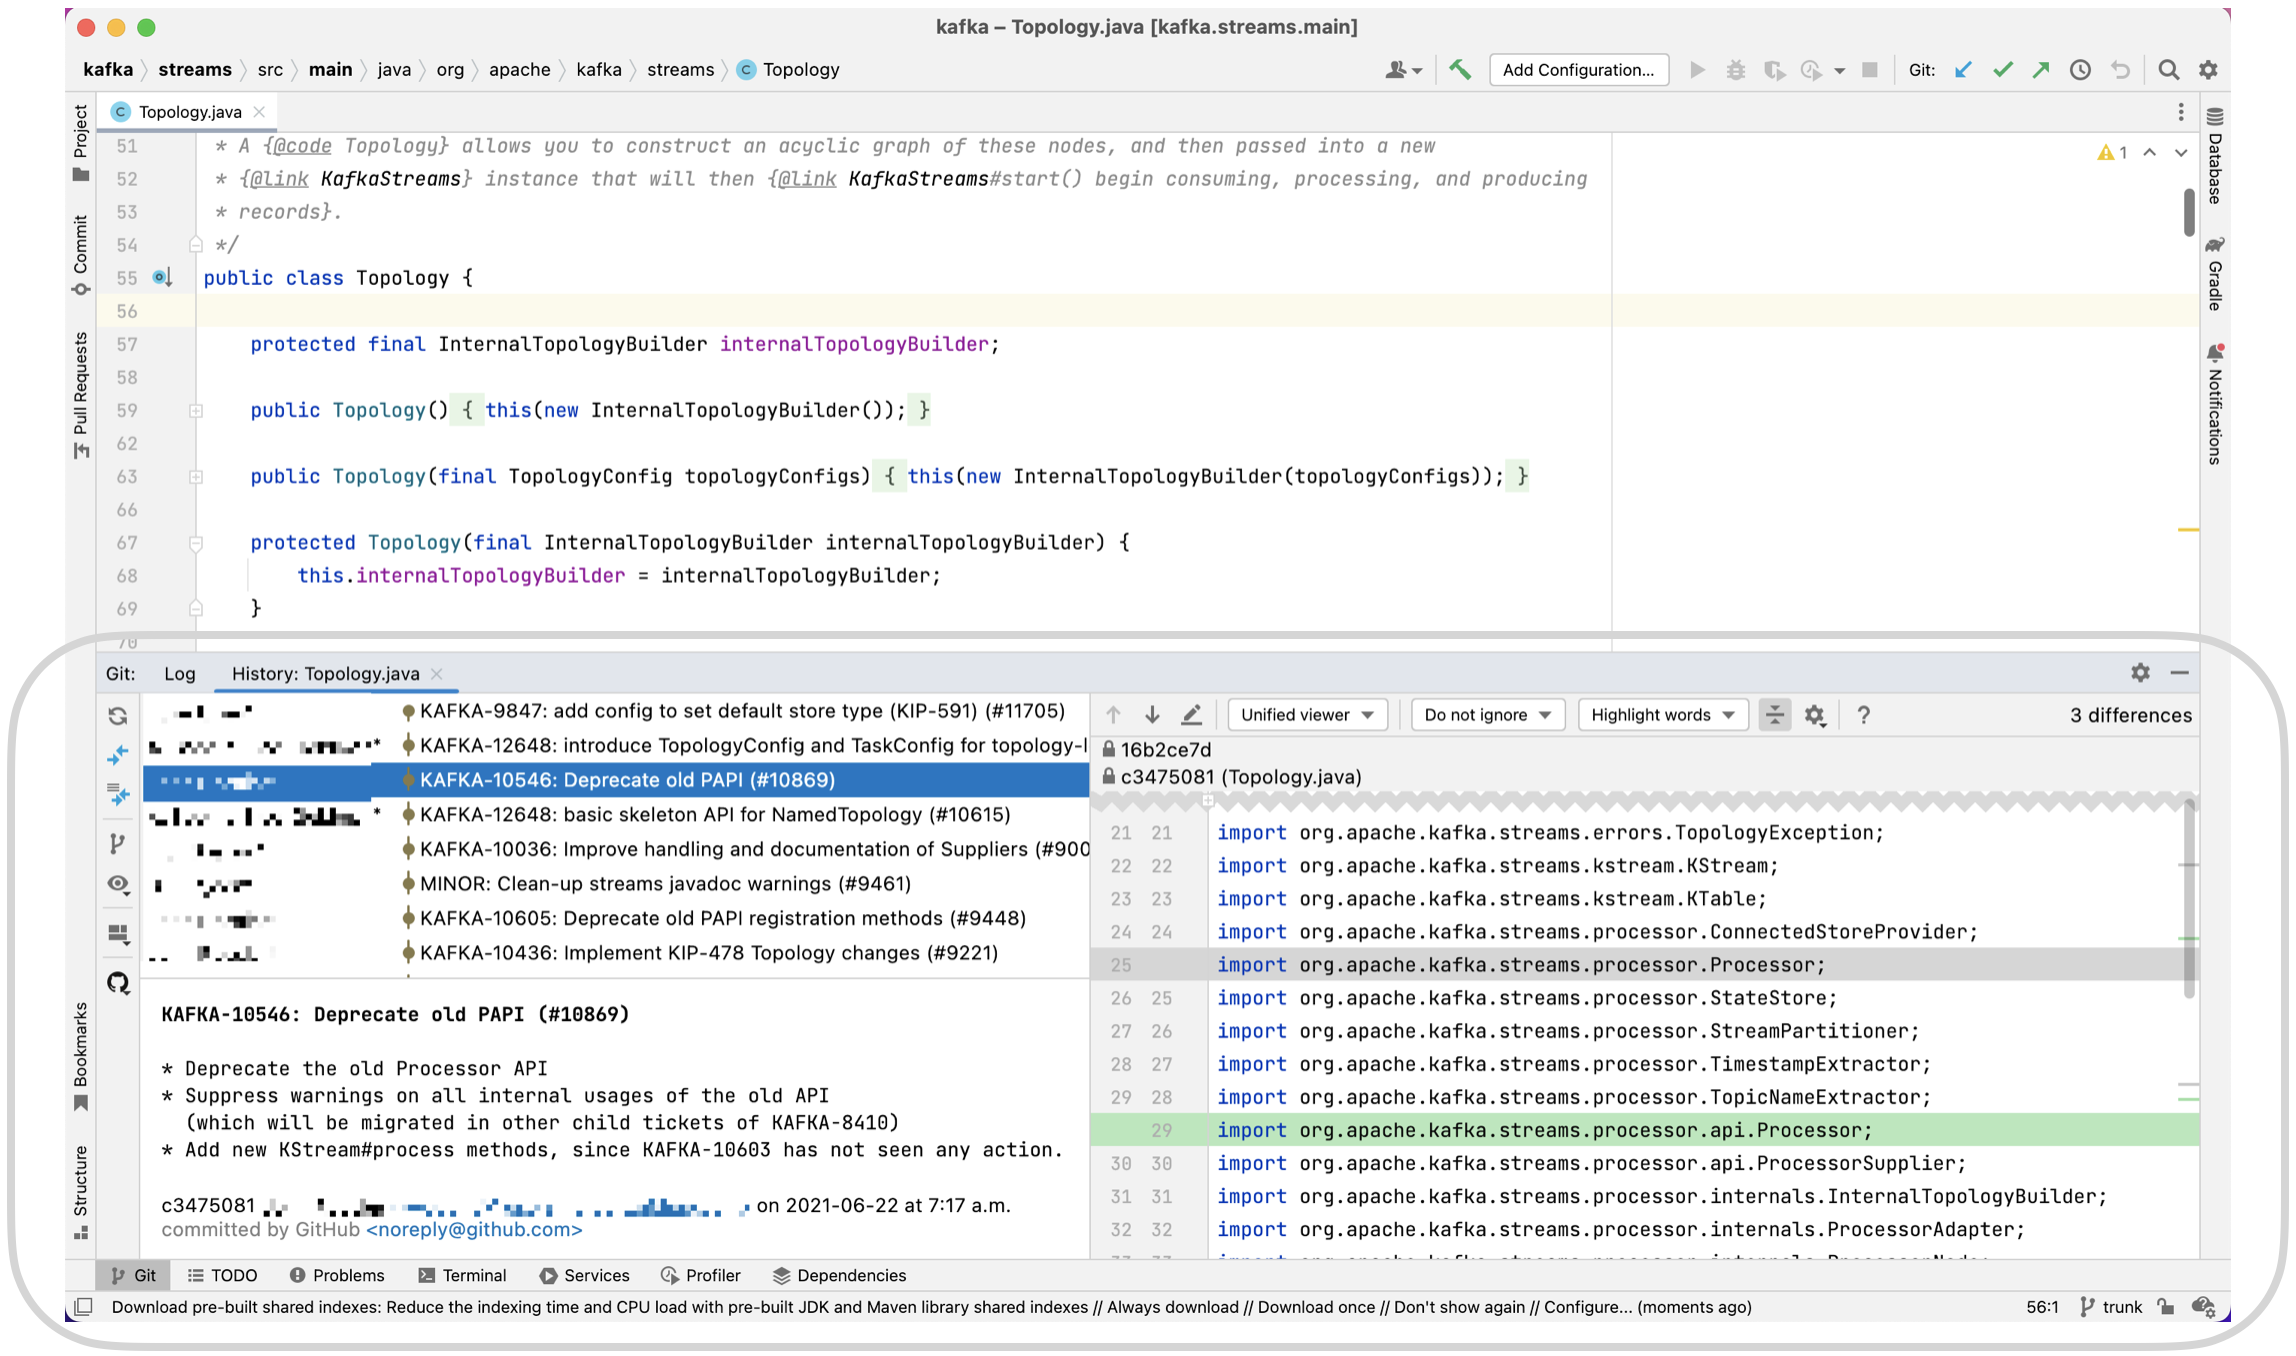
\includegraphics[width=\textwidth]{./images/intellij-overview.png}
    \caption{
        IntelliJ IDEA overview with the built-in Git client displayed on the bottom half. Shows the commit history for the \class{Topology} class in Apache Kafka.
    }
    \label{fig:IntelliJ-Overview}
\end{figure}

\begin{figure}
    \FIXME{Add annotated figure.}
    \caption{Overview of the actions added by the \toolname{Intelligent History} plugin. (A) indicates \textit{Highlight Important Changes}, (B) denotes \textit{Show Diff Metadata}, and (C) marks \textit{Show Jira Issue}.}
    \label{fig:Intelligent-History-Overview}
\end{figure}

%%%%%%%%%%%%%%%%%%%%%%%%%%%%%%%%%%%%%%%%%%%%%%%%%%%%%%%%%%%%%%%%%%%%%%
\section{Heuristics}
\label{sec:Heuristics}

For distinguishing potentially important commits from less important or trivial commits, we employ a heuristics-based approach to categorize the lines of change in a commit's diff content.
When referring to a commit's diff content, we mean the diff between the old version of a Java class in one commit, and the new version of the Java class after a commit has modified it.
This approach involves scanning the lines between commits for matches to a set of Java code patterns, which describe categories of trivial code changes.
Each pattern is expressed by a form of regular expressions.
While using regular expressions sacrifices some degree of accuracy on what is considered a ``trivial'' line of code change to a user,
regular expressions have the advantage of being lightweight in efficiency and interpretability over other approaches to detecting code changes in programs such as abstract syntax tree (\entity{AST}) matching and comparisons \cite{murphy_lightweight_1996}.
The goal of our approach is to understand if a minimal set of patterns for expressing trivial code changes can be effective at supporting a software developer in more efficiently navigating software history when searching for code rationale information.

Our approach for detecting trivial commits uses the following categories for code changes, represented by regular expressions: 

\begin{itemize}
    \item \textit{Documentation}: \dots
    \item \textit{Annotation}: \dots
    \item \textit{Import}: \dots
    \item \textit{Newline}: \dots
    \item \textit{Other}: \dots
\end{itemize}

We formulated these categories based on \dots \FIXME{Elaborate on the categories and they were formed.}

We use the \entity{java-diff-utils} \cite{java-diff-utils} library to extract the deltas between two states of a file in the form of lines. 
The library provides source lines and target lines. \FIXME{Elaborate on the diff analysis technique.}
This information for a user-selected commit is exposed in a pop-up when the user invokes the \textit{Show Diff Metadata}.
For example, \dots \FIXME{Add and reference a figure demonstrating the popup and the diff content}.

Although we formulated a fixed set of patterns specific to Java, \dots \FIXME{Consider moving this to a section on suggestions for future work? Comment on potential for user-defined patterns.}

%%%%%%%%%%%%%%%%%%%%%%%%%%%%%%%%%%%%%%%%%%%%%%%%%%%%%%%%%%%%%%%%%%%%%%
\section{Predictions}
\label{sec:Predictions}

We describe how we predict a user might be able to use the actions from \toolname{Intelligent History}.

%%%%%%%%%%%%%%%%%%%%%%%%%%%%%%%%%%%%%%%%%%%%%%%%%%%%%%%%%%%%%%%%%%%%%%
\endinput

Any text after an \endinput is ignored.
You could put scraps here or things in progress.